\documentclass[]{extarticle}
\usepackage{lmodern}
\usepackage{amssymb,amsmath}
\usepackage{ifxetex,ifluatex}
\usepackage{fixltx2e} % provides \textsubscript
\ifnum 0\ifxetex 1\fi\ifluatex 1\fi=0 % if pdftex
  \usepackage[T1]{fontenc}
  \usepackage[utf8]{inputenc}
\else % if luatex or xelatex
  \ifxetex
    \usepackage{mathspec}
  \else
    \usepackage{fontspec}
  \fi
  \defaultfontfeatures{Ligatures=TeX,Scale=MatchLowercase}
\fi
% use upquote if available, for straight quotes in verbatim environments
\IfFileExists{upquote.sty}{\usepackage{upquote}}{}
% use microtype if available
\IfFileExists{microtype.sty}{%
\usepackage{microtype}
\UseMicrotypeSet[protrusion]{basicmath} % disable protrusion for tt fonts
}{}
\usepackage[margin=0.6in]{geometry}
\usepackage{hyperref}
\hypersetup{unicode=true,
            pdftitle={Chapter 11: Multiple Regression, Pairs Plots, and Added Variable Plots},
            pdfborder={0 0 0},
            breaklinks=true}
\urlstyle{same}  % don't use monospace font for urls
\usepackage{color}
\usepackage{fancyvrb}
\newcommand{\VerbBar}{|}
\newcommand{\VERB}{\Verb[commandchars=\\\{\}]}
\DefineVerbatimEnvironment{Highlighting}{Verbatim}{commandchars=\\\{\}}
% Add ',fontsize=\small' for more characters per line
\usepackage{framed}
\definecolor{shadecolor}{RGB}{248,248,248}
\newenvironment{Shaded}{\begin{snugshade}}{\end{snugshade}}
\newcommand{\KeywordTok}[1]{\textcolor[rgb]{0.13,0.29,0.53}{\textbf{#1}}}
\newcommand{\DataTypeTok}[1]{\textcolor[rgb]{0.13,0.29,0.53}{#1}}
\newcommand{\DecValTok}[1]{\textcolor[rgb]{0.00,0.00,0.81}{#1}}
\newcommand{\BaseNTok}[1]{\textcolor[rgb]{0.00,0.00,0.81}{#1}}
\newcommand{\FloatTok}[1]{\textcolor[rgb]{0.00,0.00,0.81}{#1}}
\newcommand{\ConstantTok}[1]{\textcolor[rgb]{0.00,0.00,0.00}{#1}}
\newcommand{\CharTok}[1]{\textcolor[rgb]{0.31,0.60,0.02}{#1}}
\newcommand{\SpecialCharTok}[1]{\textcolor[rgb]{0.00,0.00,0.00}{#1}}
\newcommand{\StringTok}[1]{\textcolor[rgb]{0.31,0.60,0.02}{#1}}
\newcommand{\VerbatimStringTok}[1]{\textcolor[rgb]{0.31,0.60,0.02}{#1}}
\newcommand{\SpecialStringTok}[1]{\textcolor[rgb]{0.31,0.60,0.02}{#1}}
\newcommand{\ImportTok}[1]{#1}
\newcommand{\CommentTok}[1]{\textcolor[rgb]{0.56,0.35,0.01}{\textit{#1}}}
\newcommand{\DocumentationTok}[1]{\textcolor[rgb]{0.56,0.35,0.01}{\textbf{\textit{#1}}}}
\newcommand{\AnnotationTok}[1]{\textcolor[rgb]{0.56,0.35,0.01}{\textbf{\textit{#1}}}}
\newcommand{\CommentVarTok}[1]{\textcolor[rgb]{0.56,0.35,0.01}{\textbf{\textit{#1}}}}
\newcommand{\OtherTok}[1]{\textcolor[rgb]{0.56,0.35,0.01}{#1}}
\newcommand{\FunctionTok}[1]{\textcolor[rgb]{0.00,0.00,0.00}{#1}}
\newcommand{\VariableTok}[1]{\textcolor[rgb]{0.00,0.00,0.00}{#1}}
\newcommand{\ControlFlowTok}[1]{\textcolor[rgb]{0.13,0.29,0.53}{\textbf{#1}}}
\newcommand{\OperatorTok}[1]{\textcolor[rgb]{0.81,0.36,0.00}{\textbf{#1}}}
\newcommand{\BuiltInTok}[1]{#1}
\newcommand{\ExtensionTok}[1]{#1}
\newcommand{\PreprocessorTok}[1]{\textcolor[rgb]{0.56,0.35,0.01}{\textit{#1}}}
\newcommand{\AttributeTok}[1]{\textcolor[rgb]{0.77,0.63,0.00}{#1}}
\newcommand{\RegionMarkerTok}[1]{#1}
\newcommand{\InformationTok}[1]{\textcolor[rgb]{0.56,0.35,0.01}{\textbf{\textit{#1}}}}
\newcommand{\WarningTok}[1]{\textcolor[rgb]{0.56,0.35,0.01}{\textbf{\textit{#1}}}}
\newcommand{\AlertTok}[1]{\textcolor[rgb]{0.94,0.16,0.16}{#1}}
\newcommand{\ErrorTok}[1]{\textcolor[rgb]{0.64,0.00,0.00}{\textbf{#1}}}
\newcommand{\NormalTok}[1]{#1}
\usepackage{graphicx,grffile}
\makeatletter
\def\maxwidth{\ifdim\Gin@nat@width>\linewidth\linewidth\else\Gin@nat@width\fi}
\def\maxheight{\ifdim\Gin@nat@height>\textheight\textheight\else\Gin@nat@height\fi}
\makeatother
% Scale images if necessary, so that they will not overflow the page
% margins by default, and it is still possible to overwrite the defaults
% using explicit options in \includegraphics[width, height, ...]{}
\setkeys{Gin}{width=\maxwidth,height=\maxheight,keepaspectratio}
\IfFileExists{parskip.sty}{%
\usepackage{parskip}
}{% else
\setlength{\parindent}{0pt}
\setlength{\parskip}{6pt plus 2pt minus 1pt}
}
\setlength{\emergencystretch}{3em}  % prevent overfull lines
\providecommand{\tightlist}{%
  \setlength{\itemsep}{0pt}\setlength{\parskip}{0pt}}
\setcounter{secnumdepth}{0}
% Redefines (sub)paragraphs to behave more like sections
\ifx\paragraph\undefined\else
\let\oldparagraph\paragraph
\renewcommand{\paragraph}[1]{\oldparagraph{#1}\mbox{}}
\fi
\ifx\subparagraph\undefined\else
\let\oldsubparagraph\subparagraph
\renewcommand{\subparagraph}[1]{\oldsubparagraph{#1}\mbox{}}
\fi

%%% Use protect on footnotes to avoid problems with footnotes in titles
\let\rmarkdownfootnote\footnote%
\def\footnote{\protect\rmarkdownfootnote}

%%% Change title format to be more compact
\usepackage{titling}

% Create subtitle command for use in maketitle
\newcommand{\subtitle}[1]{
  \posttitle{
    \begin{center}\large#1\end{center}
    }
}

\setlength{\droptitle}{-2em}

  \title{Chapter 11: Multiple Regression, Pairs Plots, and Added Variable Plots}
    \pretitle{\vspace{\droptitle}\centering\huge}
  \posttitle{\par}
    \author{}
    \preauthor{}\postauthor{}
    \date{}
    \predate{}\postdate{}
  
\usepackage{soul}
\usepackage{booktabs}

\begin{document}
\maketitle

\subsection{Duncan's Occupational Prestige
Data}\label{duncans-occupational-prestige-data}

\paragraph{Intro to data}\label{intro-to-data}

We have a data set with measurements on 45 different U.S. occupations as
of 1950 (descriptions below are quotes from Fox and Weisberg, 2011):

\begin{itemize}
\tightlist
\item
  \texttt{type}: Type of occupation. A factor with the following levels:
  \texttt{prof}, professional and managerial; \texttt{wc}, white-collar;
  \texttt{bc}, blue-collar.
\item
  \texttt{income}: Percentage of occupational incumbents in the 1950 US
  Census who earned \$3,500 or more per year (about \$36,000 in 2017 US
  dollars).
\item
  \texttt{education}: Percentage of occupational incumbents in 1950 who
  were high school graduates (which, were we cynical, we would say is
  roughly equivalent to a PhD in 2017)
\item
  \texttt{prestige}: Percentage of respondents in a social survey who
  rated the occupation as ``good'' or better in prestige
\end{itemize}

\begin{Shaded}
\begin{Highlighting}[]
\KeywordTok{head}\NormalTok{(Duncan)}
\end{Highlighting}
\end{Shaded}

\begin{verbatim}
##            type income education prestige occupation
## accountant prof     62        86       82 accountant
## pilot      prof     72        76       83      pilot
## architect  prof     75        92       90  architect
## author     prof     55        90       76     author
## chemist    prof     64        86       90    chemist
## minister   prof     21        84       87   minister
\end{verbatim}

References:

\begin{itemize}
\tightlist
\item
  Fox, J. and Weisberg, S. (2011) An R Companion to Applied Regression,
  Second Edition, Sage.
\item
  Duncan, O. D. (1961) A socioeconomic index for all occupations. In
  Reiss, A. J., Jr. (Ed.) Occupations and Social Status. Free Press
  {[}Table VI-1{]}.
\end{itemize}

Let's consider a model for occupational prestige as a function of
income, education, and type of occupation.

We should always start with plots, but we're really hitting the limits
of what's plottable now\ldots{}

\newpage

\paragraph{Option 1: plotly}\label{option-1-plotly}

\begin{itemize}
\tightlist
\item
  Formatting very similar to, but not exactly the same as, ggplot2
\item
  \textbf{Can't show output in pdf, only for html output or interactive
  use}
\item
  Can't be used for any more variables than we have in this example.
\item
  If plotly code doesn't give you what you want right away, it can be
  essentially impossible to fix (not a fully developed and functional
  package).
\end{itemize}

\begin{Shaded}
\begin{Highlighting}[]
\KeywordTok{library}\NormalTok{(plotly)}
\KeywordTok{plot_ly}\NormalTok{(Duncan, }\DataTypeTok{x =} \OperatorTok{~}\NormalTok{income, }\DataTypeTok{y =} \OperatorTok{~}\NormalTok{education, }\DataTypeTok{z =} \OperatorTok{~}\NormalTok{prestige, }\DataTypeTok{color =} \OperatorTok{~}\NormalTok{type) }\OperatorTok
\StringTok{  }\KeywordTok{add_markers}\NormalTok{()}
\end{Highlighting}
\end{Shaded}

Here's a screenshot, will demo live:

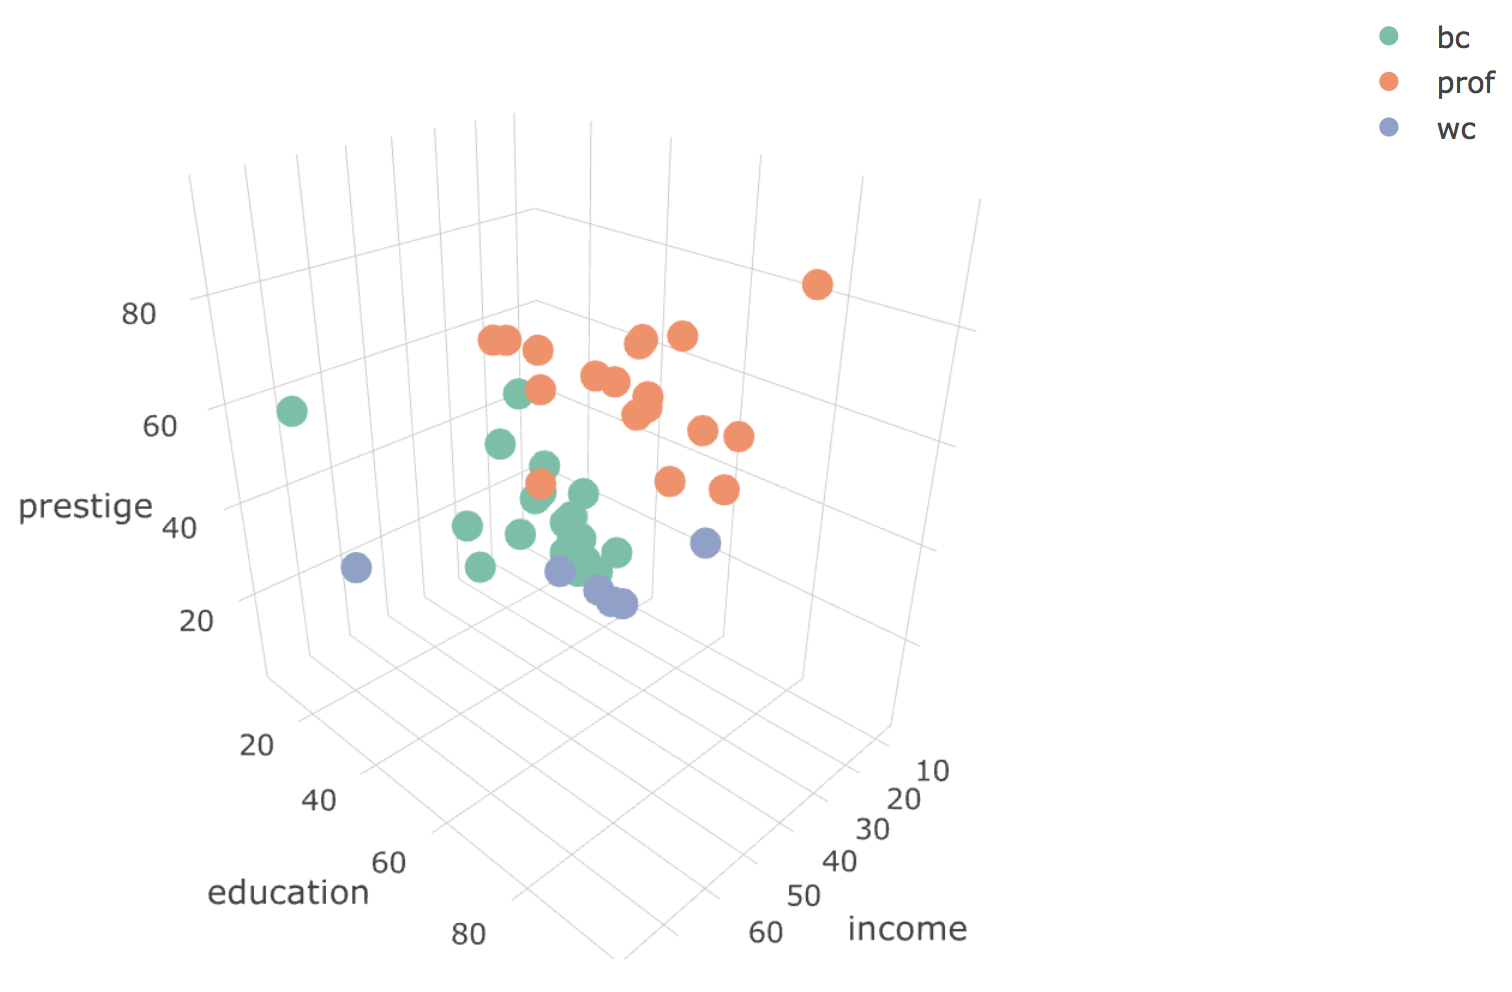
\includegraphics[height=3in]{plotly_screenshot.png}

\newpage

\paragraph{Option 2: Pairs Plots}\label{option-2-pairs-plots}

\begin{Shaded}
\begin{Highlighting}[]
\KeywordTok{library}\NormalTok{(GGally)}
\end{Highlighting}
\end{Shaded}

\begin{verbatim}
## 
## Attaching package: 'GGally'
\end{verbatim}

\begin{verbatim}
## The following object is masked from 'package:dplyr':
## 
##     nasa
\end{verbatim}

\begin{Shaded}
\begin{Highlighting}[]
\KeywordTok{ggpairs}\NormalTok{(Duncan }\OperatorTok\StringTok{ }\KeywordTok{select}\NormalTok{(}\OperatorTok{-}\NormalTok{occupation))}
\end{Highlighting}
\end{Shaded}

\begin{verbatim}
## `stat_bin()` using `bins = 30`. Pick better value with `binwidth`.
\end{verbatim}

\begin{verbatim}
## `stat_bin()` using `bins = 30`. Pick better value with `binwidth`.
## `stat_bin()` using `bins = 30`. Pick better value with `binwidth`.
\end{verbatim}

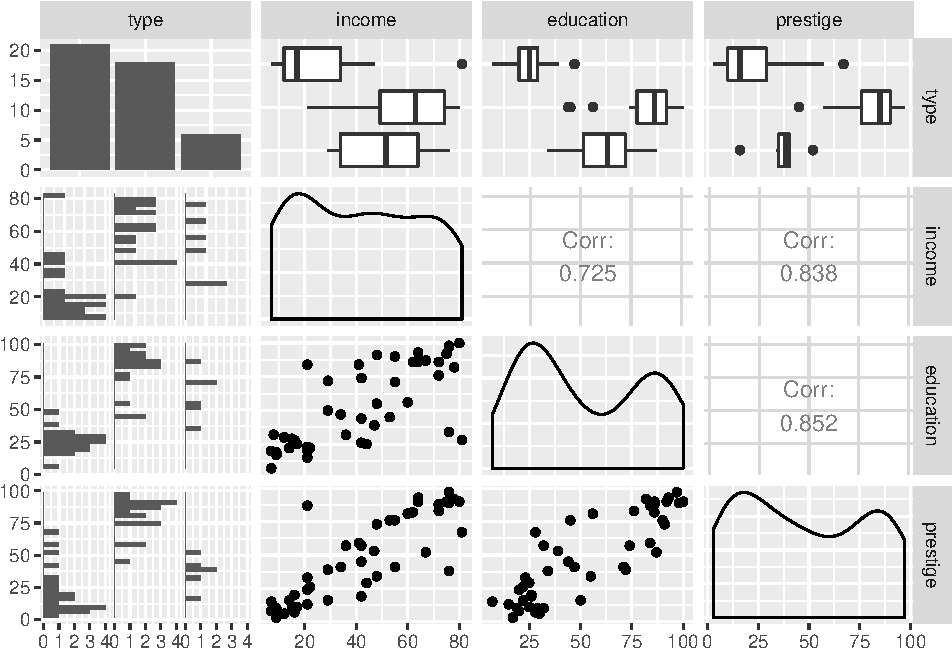
\includegraphics{20190417_avPlots_files/figure-latex/unnamed-chunk-3-1.pdf}

Possible evidence of one outlier? Let's fit some models and come back to
that later.

\newpage

\subsection{A first model - income only explanatory
variable}\label{a-first-model---income-only-explanatory-variable}

\begin{Shaded}
\begin{Highlighting}[]
\NormalTok{lm_fit_}\DecValTok{1}\NormalTok{ <-}\StringTok{ }\KeywordTok{lm}\NormalTok{(prestige }\OperatorTok{~}\StringTok{ }\NormalTok{income, }\DataTypeTok{data =}\NormalTok{ Duncan)}
\KeywordTok{summary}\NormalTok{(lm_fit_}\DecValTok{1}\NormalTok{)}
\end{Highlighting}
\end{Shaded}

\begin{verbatim}
## 
## Call:
## lm(formula = prestige ~ income, data = Duncan)
## 
## Residuals:
##     Min      1Q  Median      3Q     Max 
## -46.566  -9.421   0.257   9.167  61.855 
## 
## Coefficients:
##             Estimate Std. Error t value Pr(>|t|)    
## (Intercept)   2.4566     5.1901   0.473    0.638    
## income        1.0804     0.1074  10.062 7.14e-13 ***
## ---
## Signif. codes:  0 '***' 0.001 '**' 0.01 '*' 0.05 '.' 0.1 ' ' 1
## 
## Residual standard error: 17.4 on 43 degrees of freedom
## Multiple R-squared:  0.7019, Adjusted R-squared:  0.695 
## F-statistic: 101.3 on 1 and 43 DF,  p-value: 7.144e-13
\end{verbatim}

\begin{Shaded}
\begin{Highlighting}[]
\KeywordTok{ggplot}\NormalTok{(}\DataTypeTok{data =}\NormalTok{ Duncan, }\DataTypeTok{mapping =} \KeywordTok{aes}\NormalTok{(}\DataTypeTok{x =}\NormalTok{ income, }\DataTypeTok{y =}\NormalTok{ prestige)) }\OperatorTok{+}
\StringTok{  }\KeywordTok{geom_point}\NormalTok{() }\OperatorTok{+}
\StringTok{  }\KeywordTok{geom_smooth}\NormalTok{(}\DataTypeTok{method =} \StringTok{"lm"}\NormalTok{)}
\end{Highlighting}
\end{Shaded}

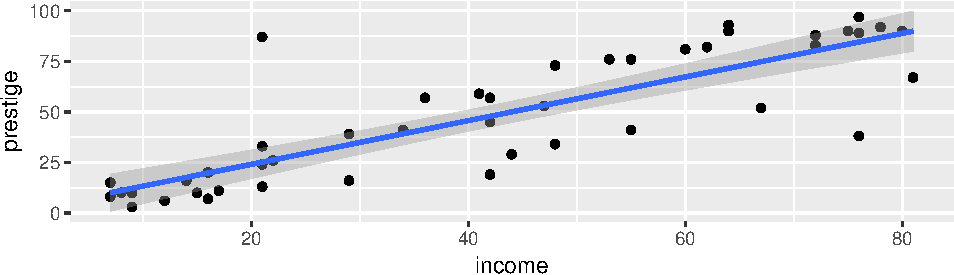
\includegraphics{20190417_avPlots_files/figure-latex/unnamed-chunk-5-1.pdf}

\paragraph{What is the equation of the estimated
line?}\label{what-is-the-equation-of-the-estimated-line}

\vspace{3cm}

\paragraph{What is the interpretation of the coefficient estimate for
income?}\label{what-is-the-interpretation-of-the-coefficient-estimate-for-income}

\newpage

\subsection{Second Model: income and education as explanatory
variables}\label{second-model-income-and-education-as-explanatory-variables}

\begin{Shaded}
\begin{Highlighting}[]
\NormalTok{lm_fit_}\DecValTok{2}\NormalTok{ <-}\StringTok{ }\KeywordTok{lm}\NormalTok{(prestige }\OperatorTok{~}\StringTok{ }\NormalTok{income }\OperatorTok{+}\StringTok{ }\NormalTok{education, }\DataTypeTok{data =}\NormalTok{ Duncan)}
\KeywordTok{summary}\NormalTok{(lm_fit_}\DecValTok{2}\NormalTok{)}
\end{Highlighting}
\end{Shaded}

\begin{verbatim}
## 
## Call:
## lm(formula = prestige ~ income + education, data = Duncan)
## 
## Residuals:
##     Min      1Q  Median      3Q     Max 
## -29.538  -6.417   0.655   6.605  34.641 
## 
## Coefficients:
##             Estimate Std. Error t value Pr(>|t|)    
## (Intercept) -6.06466    4.27194  -1.420    0.163    
## income       0.59873    0.11967   5.003 1.05e-05 ***
## education    0.54583    0.09825   5.555 1.73e-06 ***
## ---
## Signif. codes:  0 '***' 0.001 '**' 0.01 '*' 0.05 '.' 0.1 ' ' 1
## 
## Residual standard error: 13.37 on 42 degrees of freedom
## Multiple R-squared:  0.8282, Adjusted R-squared:   0.82 
## F-statistic: 101.2 on 2 and 42 DF,  p-value: < 2.2e-16
\end{verbatim}

\paragraph{What's the estimated equation of this
model?}\label{whats-the-estimated-equation-of-this-model}

\vspace{3cm}

\paragraph{This can be visualized as a
plane}\label{this-can-be-visualized-as-a-plane}

Plotly code suppressed because it's awful.

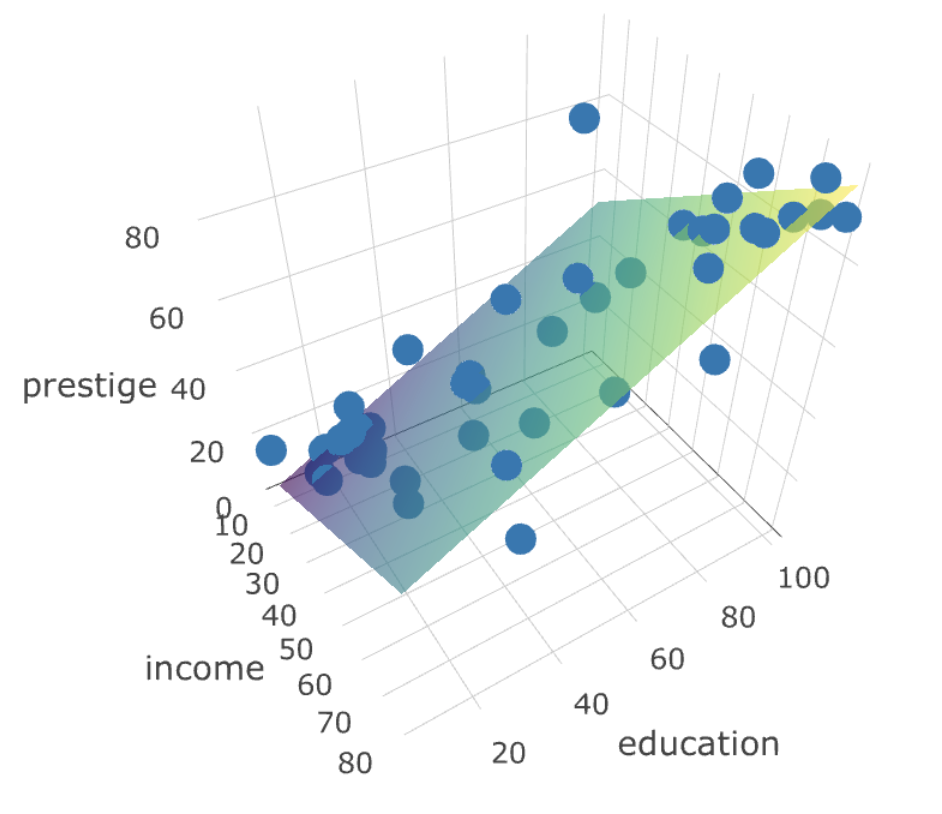
\includegraphics[height=3in]{plotly_ss_1plane.png}

\paragraph{What is the interpretation of the coefficient estimate for
income?}\label{what-is-the-interpretation-of-the-coefficient-estimate-for-income-1}

\vspace{4cm}

\paragraph{Added Variables Plots}\label{added-variables-plots}

\begin{itemize}
\tightlist
\item
  \textbf{After accounting for the effects of other variables in the
  model, what is the relationship between income and prestige?}
\item
  Focus on added variable plot for income: \textbf{after accounting for
  education},

  \begin{itemize}
  \tightlist
  \item
    New X variable is \emph{residuals} from a regression of income on
    education (what's left over in income, after accounting for
    education level?)
  \item
    New Y variable is \emph{residuals} from a regression of prestige on
    education (what's left over in prestige, after accounting for
    education level?)
  \item
    The slope of the line describing the relationship between these
    residuals is the estimated coefficient for income from the model
    fit.
  \end{itemize}
\end{itemize}

\begin{Shaded}
\begin{Highlighting}[]
\KeywordTok{library}\NormalTok{(car)}
\KeywordTok{avPlots}\NormalTok{(lm_fit_}\DecValTok{2}\NormalTok{)}
\end{Highlighting}
\end{Shaded}

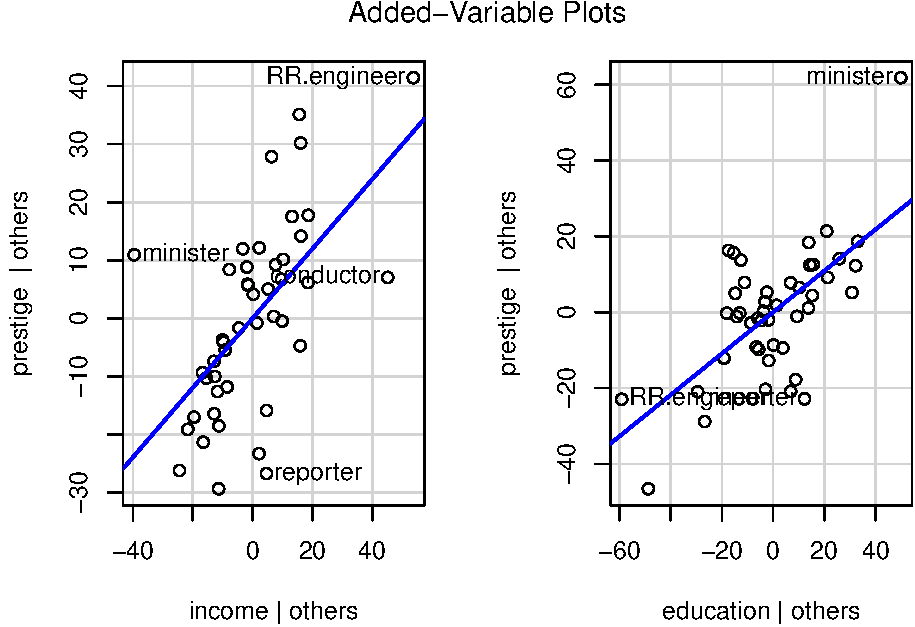
\includegraphics{20190417_avPlots_files/figure-latex/unnamed-chunk-8-1.pdf}

\begin{Shaded}
\begin{Highlighting}[]
\NormalTok{fit_income_education <-}\StringTok{ }\KeywordTok{lm}\NormalTok{(income }\OperatorTok{~}\StringTok{ }\NormalTok{education, }\DataTypeTok{data =}\NormalTok{ Duncan)}
\NormalTok{fit_prestige_educaiton <-}\StringTok{ }\KeywordTok{lm}\NormalTok{(prestige }\OperatorTok{~}\StringTok{ }\NormalTok{education, }\DataTypeTok{data =}\NormalTok{ Duncan)}
\NormalTok{av_df <-}\StringTok{ }\KeywordTok{data.frame}\NormalTok{(}
  \DataTypeTok{income_resids =} \KeywordTok{residuals}\NormalTok{(fit_income_education),}
  \DataTypeTok{prestige_resids =} \KeywordTok{residuals}\NormalTok{(fit_prestige_educaiton)}
\NormalTok{)}
\NormalTok{fit_prestige_income_accounting_education <-}\StringTok{ }\KeywordTok{lm}\NormalTok{(prestige_resids }\OperatorTok{~}\StringTok{ }\NormalTok{income_resids, }\DataTypeTok{data =}\NormalTok{ av_df)}
\KeywordTok{summary}\NormalTok{(fit_prestige_income_accounting_education)}
\end{Highlighting}
\end{Shaded}

\begin{verbatim}
## 
## Call:
## lm(formula = prestige_resids ~ income_resids, data = av_df)
## 
## Residuals:
##     Min      1Q  Median      3Q     Max 
## -29.538  -6.417   0.655   6.605  34.641 
## 
## Coefficients:
##                 Estimate Std. Error t value Pr(>|t|)    
## (Intercept)   -5.954e-16  1.970e+00   0.000        1    
## income_resids  5.987e-01  1.183e-01   5.063 8.25e-06 ***
## ---
## Signif. codes:  0 '***' 0.001 '**' 0.01 '*' 0.05 '.' 0.1 ' ' 1
## 
## Residual standard error: 13.21 on 43 degrees of freedom
## Multiple R-squared:  0.3734, Adjusted R-squared:  0.3589 
## F-statistic: 25.63 on 1 and 43 DF,  p-value: 8.246e-06
\end{verbatim}

Compare to coefficient from model with income and education as
explanatory variables.

\newpage

\subsection{Third Model: All 3 explanatory
variables!}\label{third-model-all-3-explanatory-variables}

\begin{Shaded}
\begin{Highlighting}[]
\NormalTok{lm_fit_}\DecValTok{3}\NormalTok{ <-}\StringTok{ }\KeywordTok{lm}\NormalTok{(prestige }\OperatorTok{~}\StringTok{ }\NormalTok{income }\OperatorTok{+}\StringTok{ }\NormalTok{education }\OperatorTok{+}\StringTok{ }\NormalTok{type, }\DataTypeTok{data =}\NormalTok{ Duncan)}
\KeywordTok{summary}\NormalTok{(lm_fit_}\DecValTok{3}\NormalTok{)}
\end{Highlighting}
\end{Shaded}

\begin{verbatim}
## 
## Call:
## lm(formula = prestige ~ income + education + type, data = Duncan)
## 
## Residuals:
##     Min      1Q  Median      3Q     Max 
## -14.890  -5.740  -1.754   5.442  28.972 
## 
## Coefficients:
##              Estimate Std. Error t value Pr(>|t|)    
## (Intercept)  -0.18503    3.71377  -0.050  0.96051    
## income        0.59755    0.08936   6.687 5.12e-08 ***
## education     0.34532    0.11361   3.040  0.00416 ** 
## typeprof     16.65751    6.99301   2.382  0.02206 *  
## typewc      -14.66113    6.10877  -2.400  0.02114 *  
## ---
## Signif. codes:  0 '***' 0.001 '**' 0.01 '*' 0.05 '.' 0.1 ' ' 1
## 
## Residual standard error: 9.744 on 40 degrees of freedom
## Multiple R-squared:  0.9131, Adjusted R-squared:  0.9044 
## F-statistic:   105 on 4 and 40 DF,  p-value: < 2.2e-16
\end{verbatim}

Plotly code suppressed because it's awful.

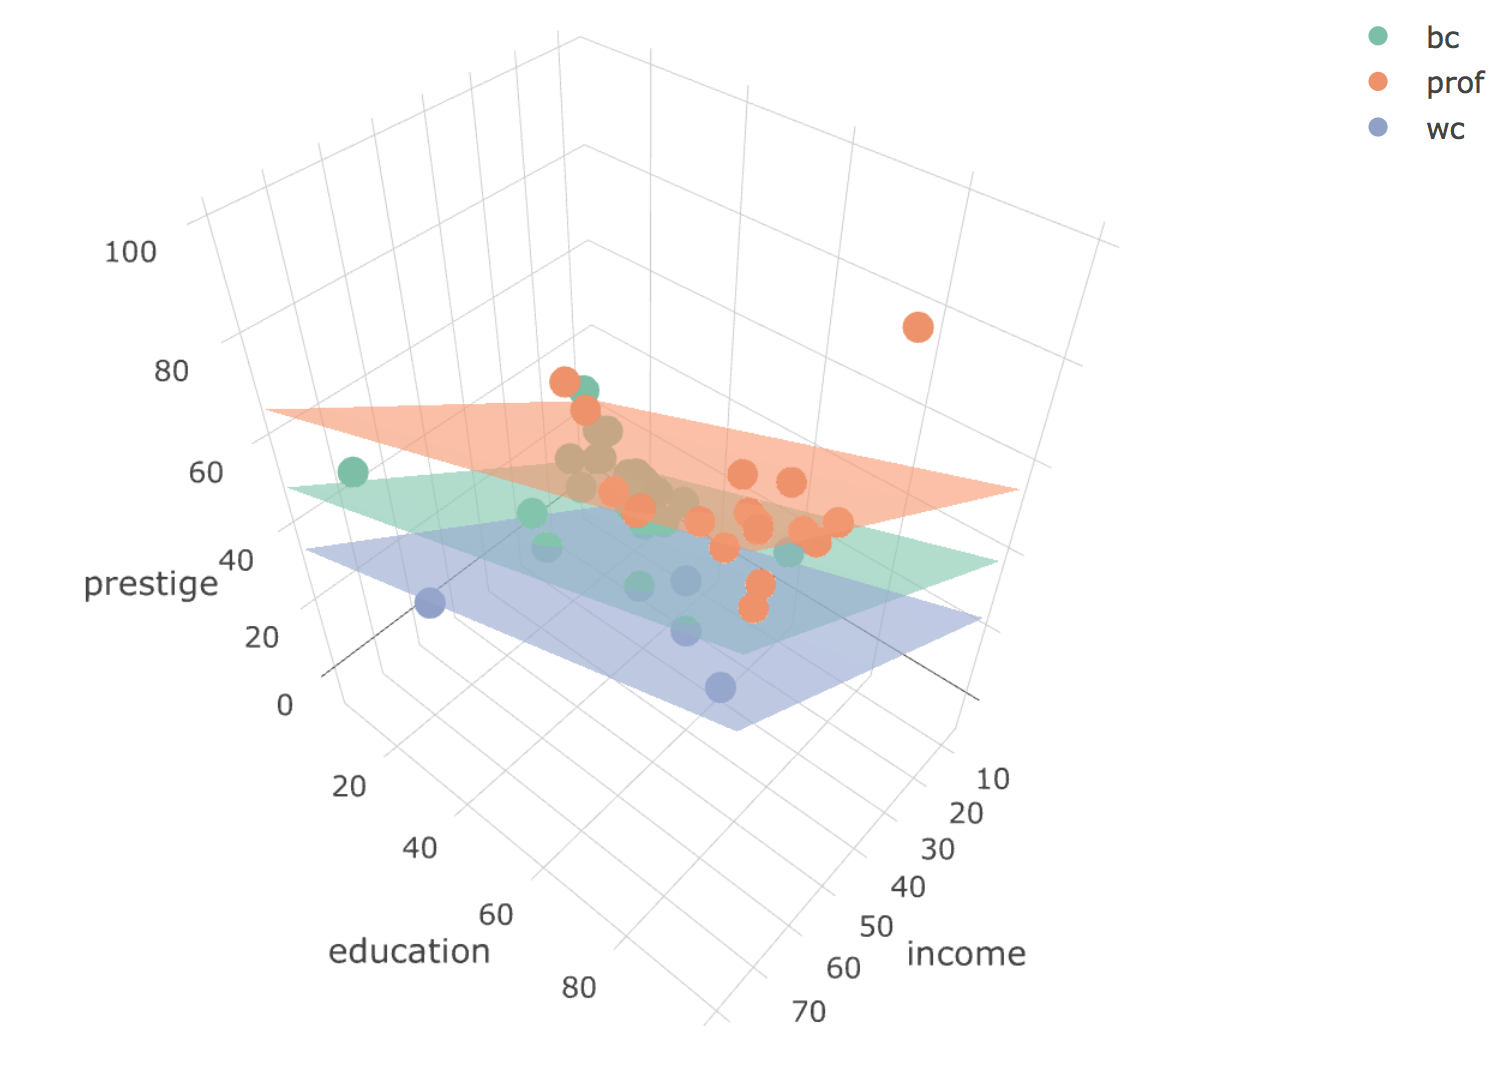
\includegraphics[height=3in]{plotly_ss_3planes.png}

\paragraph{What is the equation of the model
fit?}\label{what-is-the-equation-of-the-model-fit}

\vspace{3cm}

\paragraph{What is the interpretation of the estimated coefficient for
income?}\label{what-is-the-interpretation-of-the-estimated-coefficient-for-income}

\vspace{3cm}

\paragraph{Diagnostic Plots}\label{diagnostic-plots}

\begin{Shaded}
\begin{Highlighting}[]
\NormalTok{Duncan <-}\StringTok{ }\NormalTok{Duncan }\OperatorTok
\StringTok{  }\KeywordTok{mutate}\NormalTok{(}
    \DataTypeTok{obs_index =} \KeywordTok{row_number}\NormalTok{(),}
    \DataTypeTok{h =} \KeywordTok{hatvalues}\NormalTok{(lm_fit_}\DecValTok{3}\NormalTok{),}
    \DataTypeTok{studres =} \KeywordTok{rstudent}\NormalTok{(lm_fit_}\DecValTok{3}\NormalTok{),}
    \DataTypeTok{D =} \KeywordTok{cooks.distance}\NormalTok{(lm_fit_}\DecValTok{3}\NormalTok{)}
\NormalTok{  )}

\KeywordTok{ggplot}\NormalTok{(}\DataTypeTok{data =}\NormalTok{ Duncan, }\DataTypeTok{mapping =} \KeywordTok{aes}\NormalTok{(}\DataTypeTok{x =}\NormalTok{ obs_index, }\DataTypeTok{y =}\NormalTok{ h)) }\OperatorTok{+}
\StringTok{  }\KeywordTok{geom_point}\NormalTok{() }\OperatorTok{+}
\StringTok{  }\KeywordTok{geom_hline}\NormalTok{(}\DataTypeTok{yintercept =} \DecValTok{2} \OperatorTok{*}\StringTok{ }\DecValTok{5} \OperatorTok{/}\StringTok{ }\KeywordTok{nrow}\NormalTok{(Duncan)) }\OperatorTok{+}
\StringTok{  }\KeywordTok{ylim}\NormalTok{(}\DecValTok{0}\NormalTok{, }\DecValTok{1}\NormalTok{) }\OperatorTok{+}
\StringTok{  }\KeywordTok{ggtitle}\NormalTok{(}\StringTok{"Leverage"}\NormalTok{)}
\end{Highlighting}
\end{Shaded}

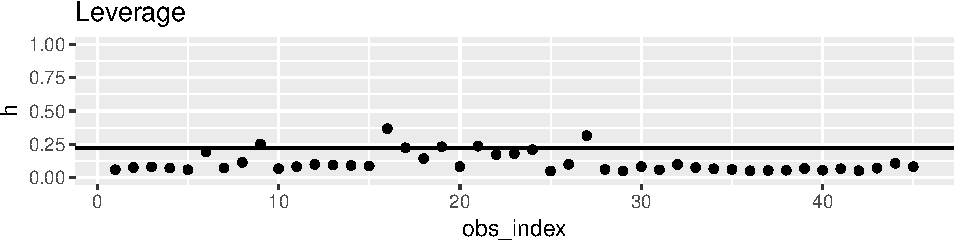
\includegraphics{20190417_avPlots_files/figure-latex/unnamed-chunk-12-1.pdf}

\begin{Shaded}
\begin{Highlighting}[]
\KeywordTok{ggplot}\NormalTok{(}\DataTypeTok{data =}\NormalTok{ Duncan, }\DataTypeTok{mapping =} \KeywordTok{aes}\NormalTok{(}\DataTypeTok{x =}\NormalTok{ obs_index, }\DataTypeTok{y =}\NormalTok{ studres)) }\OperatorTok{+}
\StringTok{  }\KeywordTok{geom_point}\NormalTok{() }\OperatorTok{+}
\StringTok{  }\KeywordTok{ggtitle}\NormalTok{(}\StringTok{"Studentized Residuals"}\NormalTok{)}
\end{Highlighting}
\end{Shaded}

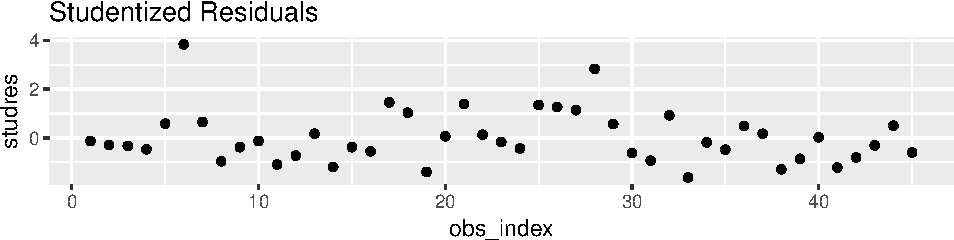
\includegraphics{20190417_avPlots_files/figure-latex/unnamed-chunk-12-2.pdf}

\begin{Shaded}
\begin{Highlighting}[]
\KeywordTok{ggplot}\NormalTok{(}\DataTypeTok{data =}\NormalTok{ Duncan, }\DataTypeTok{mapping =} \KeywordTok{aes}\NormalTok{(}\DataTypeTok{x =}\NormalTok{ obs_index, }\DataTypeTok{y =}\NormalTok{ D)) }\OperatorTok{+}
\StringTok{  }\KeywordTok{geom_point}\NormalTok{() }\OperatorTok{+}
\StringTok{  }\KeywordTok{ggtitle}\NormalTok{(}\StringTok{"Cook's Distance"}\NormalTok{)}
\end{Highlighting}
\end{Shaded}

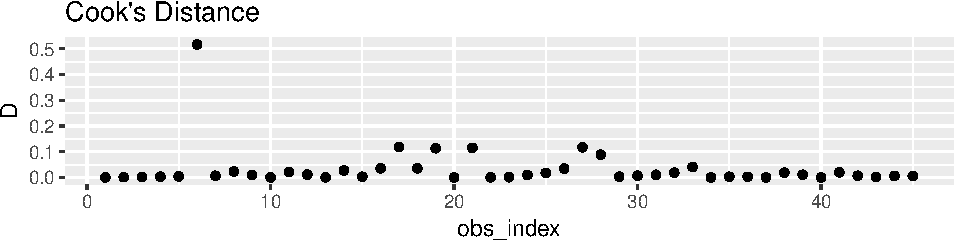
\includegraphics{20190417_avPlots_files/figure-latex/unnamed-chunk-12-3.pdf}

\begin{Shaded}
\begin{Highlighting}[]
\NormalTok{obs_to_investigate <-}\StringTok{ }\KeywordTok{c}\NormalTok{(}\DecValTok{6}\NormalTok{, }\DecValTok{16}\NormalTok{, }\DecValTok{27}\NormalTok{)}
\end{Highlighting}
\end{Shaded}

\newpage

\begin{Shaded}
\begin{Highlighting}[]
\NormalTok{Duncan[obs_to_investigate, ]}
\end{Highlighting}
\end{Shaded}

\begin{verbatim}
##    type income education prestige  occupation obs_index         h
## 6  prof     21        84       87    minister         6 0.1912053
## 16   wc     76        34       38   conductor        16 0.3663519
## 27   bc     81        28       67 RR.engineer        27 0.3146829
##       studres          D
## 6   3.8293960 0.51680533
## 16 -0.5505711 0.03567303
## 27  1.1339763 0.11725367
\end{verbatim}

\begin{Shaded}
\begin{Highlighting}[]
\KeywordTok{plot}\NormalTok{(lm_fit_}\DecValTok{3}\NormalTok{)}
\end{Highlighting}
\end{Shaded}

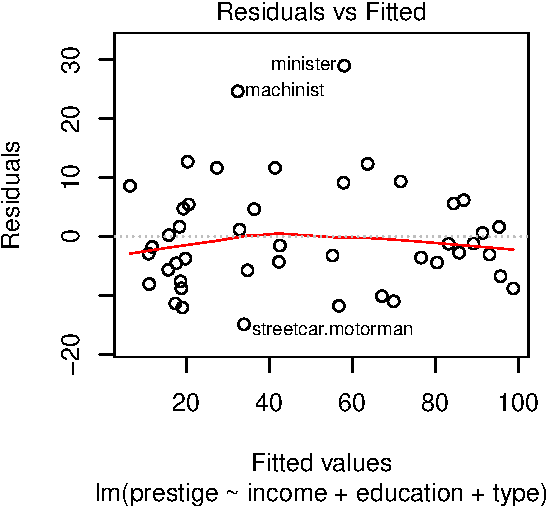
\includegraphics{20190417_avPlots_files/figure-latex/unnamed-chunk-15-1.pdf}
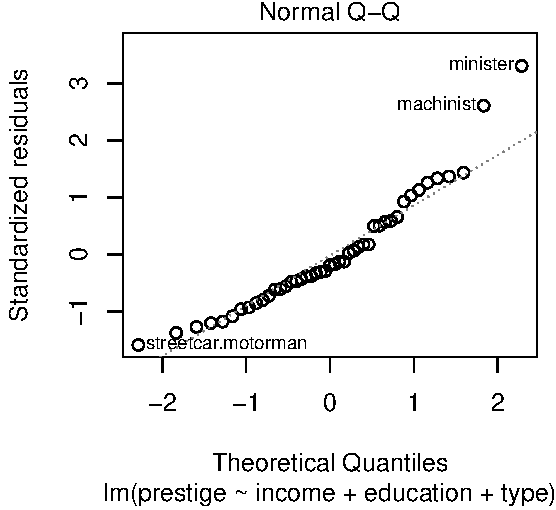
\includegraphics{20190417_avPlots_files/figure-latex/unnamed-chunk-15-2.pdf}
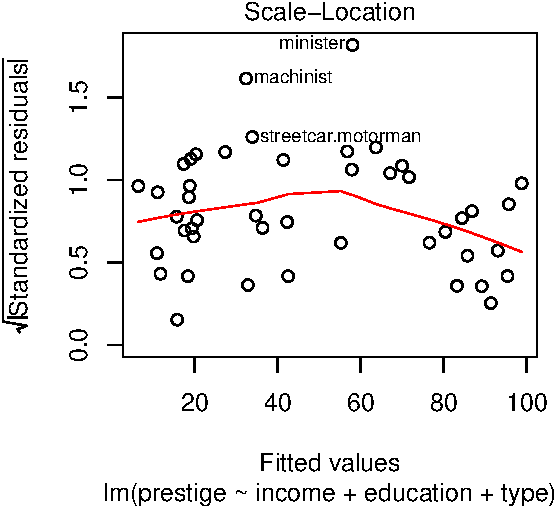
\includegraphics{20190417_avPlots_files/figure-latex/unnamed-chunk-15-3.pdf}
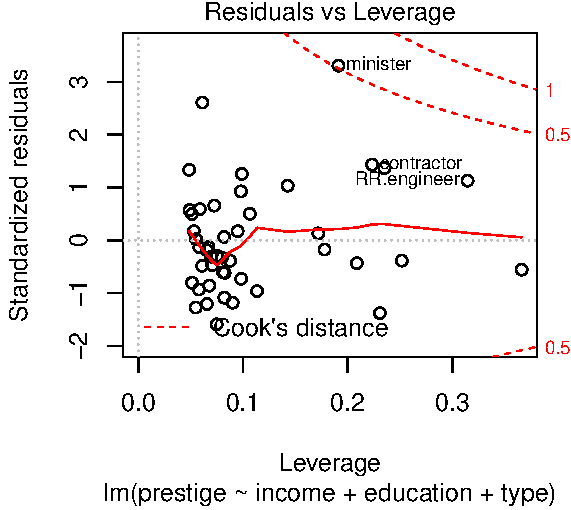
\includegraphics{20190417_avPlots_files/figure-latex/unnamed-chunk-15-4.pdf}

\newpage

\begin{Shaded}
\begin{Highlighting}[]
\NormalTok{Duncan_minus_suspicious <-}\StringTok{ }\NormalTok{Duncan[}\OperatorTok{-}\NormalTok{obs_to_investigate, ]}
\NormalTok{lm_fit_without_suspicious <-}\StringTok{ }\KeywordTok{lm}\NormalTok{(prestige }\OperatorTok{~}\StringTok{ }\NormalTok{income }\OperatorTok{+}\StringTok{ }\NormalTok{education }\OperatorTok{+}\StringTok{ }\NormalTok{type, }\DataTypeTok{data =}\NormalTok{ Duncan_minus_suspicious)}
\KeywordTok{summary}\NormalTok{(lm_fit_without_suspicious)}
\end{Highlighting}
\end{Shaded}

\begin{verbatim}
## 
## Call:
## lm(formula = prestige ~ income + education + type, data = Duncan_minus_suspicious)
## 
## Residuals:
##      Min       1Q   Median       3Q      Max 
## -18.0415  -5.3802  -0.6189   5.0992  23.2906 
## 
## Coefficients:
##             Estimate Std. Error t value Pr(>|t|)    
## (Intercept)  -1.1053     3.2745  -0.338   0.7376    
## income        0.7733     0.1171   6.607 9.53e-08 ***
## education     0.2180     0.1174   1.857   0.0714 .  
## typeprof     15.2512     6.4123   2.378   0.0227 *  
## typewc      -12.3622     5.9478  -2.078   0.0447 *  
## ---
## Signif. codes:  0 '***' 0.001 '**' 0.01 '*' 0.05 '.' 0.1 ' ' 1
## 
## Residual standard error: 8.432 on 37 degrees of freedom
## Multiple R-squared:  0.9368, Adjusted R-squared:   0.93 
## F-statistic: 137.1 on 4 and 37 DF,  p-value: < 2.2e-16
\end{verbatim}

\begin{Shaded}
\begin{Highlighting}[]
\NormalTok{Duncan_minus_minister <-}\StringTok{ }\NormalTok{Duncan[}\OperatorTok{-}\DecValTok{6}\NormalTok{, ]}
\NormalTok{lm_fit_without_minister <-}\StringTok{ }\KeywordTok{lm}\NormalTok{(prestige }\OperatorTok{~}\StringTok{ }\NormalTok{income }\OperatorTok{+}\StringTok{ }\NormalTok{education }\OperatorTok{+}\StringTok{ }\NormalTok{type, }\DataTypeTok{data =}\NormalTok{ Duncan_minus_minister)}
\KeywordTok{summary}\NormalTok{(lm_fit_without_minister)}
\end{Highlighting}
\end{Shaded}

\begin{verbatim}
## 
## Call:
## lm(formula = prestige ~ income + education + type, data = Duncan_minus_minister)
## 
## Residuals:
##      Min       1Q   Median       3Q      Max 
## -17.0521  -6.4105  -0.7819   4.6552  23.5212 
## 
## Coefficients:
##              Estimate Std. Error t value Pr(>|t|)    
## (Intercept)  -1.62984    3.22841  -0.505  0.61651    
## income        0.71813    0.08332   8.619 1.44e-10 ***
## education     0.28924    0.09917   2.917  0.00584 ** 
## typeprof     13.43111    6.09592   2.203  0.03355 *  
## typewc      -15.87744    5.28357  -3.005  0.00462 ** 
## ---
## Signif. codes:  0 '***' 0.001 '**' 0.01 '*' 0.05 '.' 0.1 ' ' 1
## 
## Residual standard error: 8.413 on 39 degrees of freedom
## Multiple R-squared:  0.9344, Adjusted R-squared:  0.9277 
## F-statistic:   139 on 4 and 39 DF,  p-value: < 2.2e-16
\end{verbatim}

\begin{Shaded}
\begin{Highlighting}[]
\NormalTok{Duncan <-}\StringTok{ }\NormalTok{Duncan }\OperatorTok
\StringTok{  }\KeywordTok{mutate}\NormalTok{(}
    \DataTypeTok{suspicious =} \KeywordTok{ifelse}\NormalTok{(}\KeywordTok{row_number}\NormalTok{() }\OperatorTok\StringTok{ }\NormalTok{obs_to_investigate, }\StringTok{"suspicious"}\NormalTok{, }\StringTok{"seems ok"}\NormalTok{)}
\NormalTok{  )}

\KeywordTok{ggplot}\NormalTok{(}\DataTypeTok{data =}\NormalTok{ Duncan, }\DataTypeTok{mapping =} \KeywordTok{aes}\NormalTok{(}\DataTypeTok{x =}\NormalTok{ education, }\DataTypeTok{y =}\NormalTok{ income, }\DataTypeTok{color =}\NormalTok{ suspicious)) }\OperatorTok{+}
\StringTok{  }\KeywordTok{geom_point}\NormalTok{()}
\end{Highlighting}
\end{Shaded}

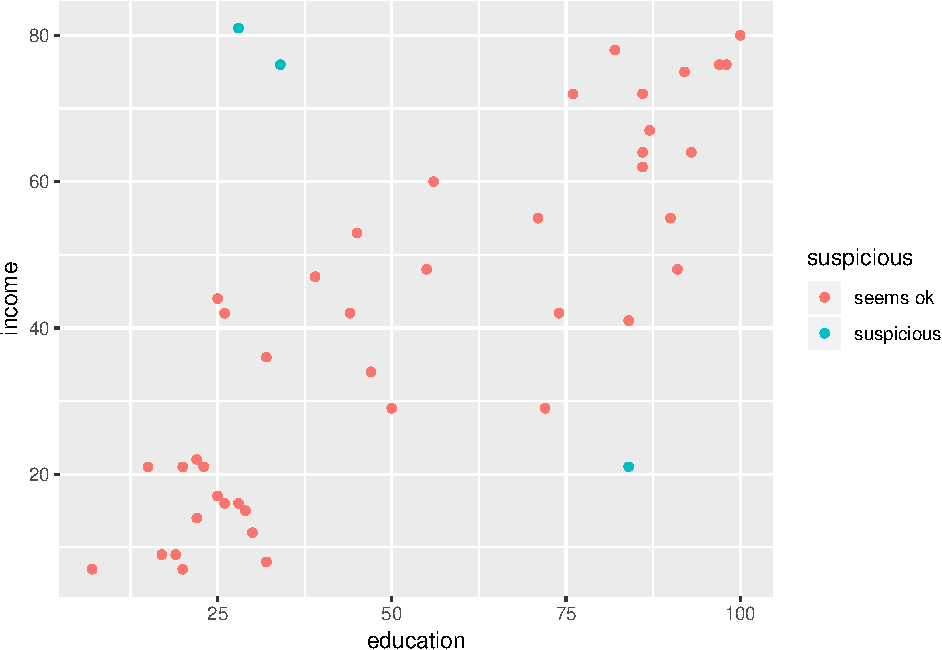
\includegraphics{20190417_avPlots_files/figure-latex/unnamed-chunk-18-1.pdf}

\paragraph{What do we say?}\label{what-do-we-say}


\end{document}
